% arara: lualatex
% arara: lualatex
% Typeset using lualatex

\documentclass{../tutorial}

\title{Traffic lights with MicroPython on \abbr{ESP32}}

\begin{document}

\begin{enumerate}

\item
    You will need a set-up environment and an \abbr{ESP32} board
    with an \abbr{RGB} \abbr{LED} stripe.

\section{Some theory}

\item
    Trough one of the microcontroller's \emph{pins},
    you can control an \abbr{RGB} \abbr{LED} strip.
    The strip you have consist of 8 cells,
    each containing 3 LEDs: red, green and blue.

    Each of those LEDs can vary in intensity from \lstinline|0| to \lstinline|255|
    and by combining them, you can show a lot of colors.
    This roughly matches what the human eye can distinguish,
    so it has been called the \emph{True Color}.

    We'll limit the light intensity to `0` to `10` so it doesn't blind you.
    If you go beyond that, cover the strip with a \emph{diffuser} such as
    a piece of paper.

\section{Controlling an \abbr{RGB} \abbr{LED} stripe}

\item
    MicroPython on the \abbr{ESP32} board already has a high-level class for
    our LED stripe, called \lstinline|NeoPixel|. Import it:

    \begin{lstlisting}
    from machine import Pin
    from neopixel import NeoPixel
    \end{lstlisting}

    In order to setup a \lstinline|NeoPixel| instance,
    you'll need to provide an output data pin \#15 and the number of cells.

    \begin{lstlisting}
    datapin = Pin(15, Pin.OUT)
    np = NeoPixel(datapin, 8)
    \end{lstlisting}

\item
    Write Red/Green/Blue triplets to the object as if it were a list of length 8.
    To make the \abbr{LED}s actually change their color,
    use the \lstinline|np.write()| method:

    \newcommand\rgb[3]{\texttt{%
        \textcolor{red}{#1},
        \textcolor{black!50!green}{#2},
        \textcolor{blue}{#3}}
    }
    \begin{lstlisting}[escapeinside=<>]
    np[0] = <\rgb{0}{5}{10}>   # green + blue = cyan
    np[1] = <\rgb{7}{1}{10}>   # red + blue = purple
    ...
    np[7] = <\rgb{10}{10}{10}> # white
    np.write()
    \end{lstlisting}

\item
    Get yourself familiarized with the stripe and how is it controlled.
    How do you turn a cell off?
    How do you get yellow light?

\section{A traffic light}

\item
    Let's design a traffic light.
    First, think how a traffic light looks like:
    It consists of 3 lights, from top to bottom:
    \begin{tikzpicture}[overlay]
        \path[use as bounding box] (-\textwidth,0) (0,0);
        \node[below left] {
\includegraphics[width=1cm]{traffic_light}};
    \end{tikzpicture}

    \begin{enumerate}
    \item red,
    \item yellow,
    \item green.
    \end{enumerate}

    Pick 3 LED cells in a row.
    Decide where is the top and where is the bottom.

    Make them all shine in their respective colors.

\item
    Create an infinite loop that simulates a traffic light.
    This light sequence is used in the Czech Republic:

    \begin{enumerate}
    \item red: cars are stopped,
    \item red \& yellow: get ready,
    \item green: cars should go,
    \item yellow: cars should stop.
    \item (repeat)
    \end{enumerate}

    Usually, the yellow phases are quite a bit shorter than
    the red and green ones.

    Use the \lstinline|sleep| function from the \lstinline|time| module:

    \begin{lstlisting}
    from time import sleep
    sleep(1)  # delay for one second
    \end{lstlisting}

    Don't forget to turn off the lights that are not used at the moment.

\item
    You've made it!
    Get yourself some swag reward from the booth staff and turn the page over.

\clearpage

\section{A railroad crossing}

    Let's design a railroad crossing signal.

    You'll need an \abbr{ESP32} board with an \abbr{RGB} \abbr{LED} stripe
    \emph{and} a servo motor.

    If you haven't controlled servos yet, \textbf{do that activity first}.

\item
    First, think how railroad crossing signalization looks and functions.
    It consists of:
    \begin{tikzpicture}[overlay]
        \path[use as bounding box] (-\textwidth,0) (0,0);
        \node[below] {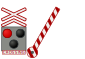
\includegraphics[width=5cm]{train}};
    \end{tikzpicture}

    \begin{itemize}
    \item 2 red lights on the top,
    \item 1 white light on the bottom,
    \item a number of gates, usually 2 or 4.
    \end{itemize}

    This is how it works in the Czech Republic:

    \begin{enumerate}
    \item white blinks (cars, cyclists or pedestrians can go),
    \item white is replaced by alternating blinking reds
          (everybody should stop),
    \item the gate(s) go down,
    \item one or more trains pass,
    \item the gate(s) go up,
    \item reds turn off,
    \item (repeat)
    \end{enumerate}

    Take in mind that you need some time before lowering the gate,
    or accidents can happen.

\item
    Pick 3 LED cells.
    Either have them in a row or get creative and carefully twist the stripe
    to create 2 rows.
    Decide which cells represent what lights.
    For starters, make them all shine in their respective colors.

\item
    Create an infinite loop that simulates the signal lights.

\item
    Add the gate – a servo motor – to the railroad crossing's sequence.
    Remember you can use PWM to turn a servo:

    \begin{lstlisting}
    from machine import Pin, PWM

    servopin = Pin(17, Pin.OUT)
    pwm = PWM(servopin, freq=50, duty=50)
    \end{lstlisting}

    To control the angle of your servomotor, set duty from 50 to 100.
    Find the numbers that work best for your gate.

    \begin{lstlisting}
    pwm.duty(75)  # use 50..100 only
    \end{lstlisting}

    Don't forget to wait between starting the red lights and putting the gate down –
    you don't want anybody to get hurt.

\item
    You rock! Isn't this awesome?

    Please return the board when you're done experimenting.

\end{enumerate}
\end{document}
